% Lotka--Volterra evaluation protocol: what is trained on, what is scored, what is stress-tested.
\documentclass[tikz,border=4pt]{standalone}
\usepackage{amsmath,amssymb}
\usepackage{mathptmx}
\usepackage[scaled=0.90]{helvet}
\usetikzlibrary{arrows.meta,decorations.pathreplacing,calc}

\definecolor{ink}{RGB}{28,32,38}
\definecolor{primary}{RGB}{155,26,32}
\definecolor{accentsoft}{RGB}{247,228,229}
\definecolor{rule}{RGB}{209,213,219}
\definecolor{blueacc}{RGB}{30,90,168}
\definecolor{bluesoft}{RGB}{232,239,248}
\definecolor{muted}{RGB}{95,107,122}

\begin{document}
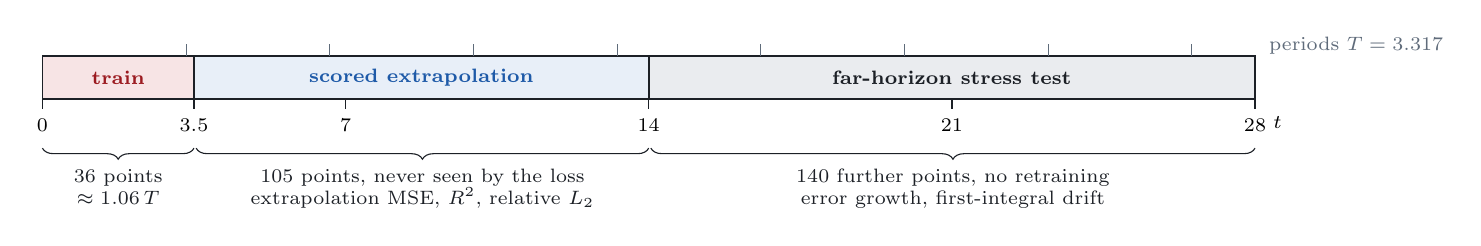
\begin{tikzpicture}[font=\sffamily\small, x=0.55cm]
% segments
\fill[accentsoft] (0,0) rectangle (3.5,0.55);
\fill[bluesoft] (3.5,0) rectangle (14,0.55);
\fill[rule!45] (14,0) rectangle (28,0.55);
\draw[ink, line width=0.6pt] (0,0) rectangle (28,0.55);
\draw[ink, line width=0.6pt] (3.5,0) -- (3.5,0.55) (14,0) -- (14,0.55);
\node[font=\scriptsize\bfseries, text=primary] at (1.75,0.275) {train};
\node[font=\scriptsize\bfseries, text=blueacc] at (8.75,0.275) {scored extrapolation};
\node[font=\scriptsize\bfseries, text=ink] at (21,0.275) {far-horizon stress test};
% ticks
\foreach \t in {0,3.5,7,14,21,28} {
  \draw[ink, line width=0.5pt] (\t,0) -- (\t,-0.12);
  \node[font=\scriptsize, anchor=north] at (\t,-0.12) {$\t$};
}
\node[font=\scriptsize, anchor=north west] at (28.2,-0.1) {$t$};
% period marks
\foreach \k in {1,...,8} {
  \pgfmathsetmacro{\tp}{\k*3.31746}
  \draw[muted, line width=0.4pt] (\tp,0.55) -- (\tp,0.7);
}
\node[font=\scriptsize, text=muted, anchor=south west] at (28.1,0.45) {periods $T=3.317$};
% braces with counts
\draw[decorate, decoration={brace, amplitude=4pt, mirror}, ink] (0,-0.62) -- (3.5,-0.62)
  node[midway, below=4pt, font=\scriptsize, align=center] {36 points\\$\approx1.06\,T$};
\draw[decorate, decoration={brace, amplitude=4pt, mirror}, ink] (3.55,-0.62) -- (14,-0.62)
  node[midway, below=4pt, font=\scriptsize, align=center] {105 points, never seen by the loss\\extrapolation MSE, $R^2$, relative $L_2$};
\draw[decorate, decoration={brace, amplitude=4pt, mirror}, ink] (14.05,-0.62) -- (28,-0.62)
  node[midway, below=4pt, font=\scriptsize, align=center] {140 further points, no retraining\\error growth, first-integral drift};
\end{tikzpicture}
\end{document}
